
\section{Teaching in a Digital Age}

\begin{frame}
  \centering
  From heavy note taking sessions\dots \\
  \begin{minipage}{0.55\linewidth}
    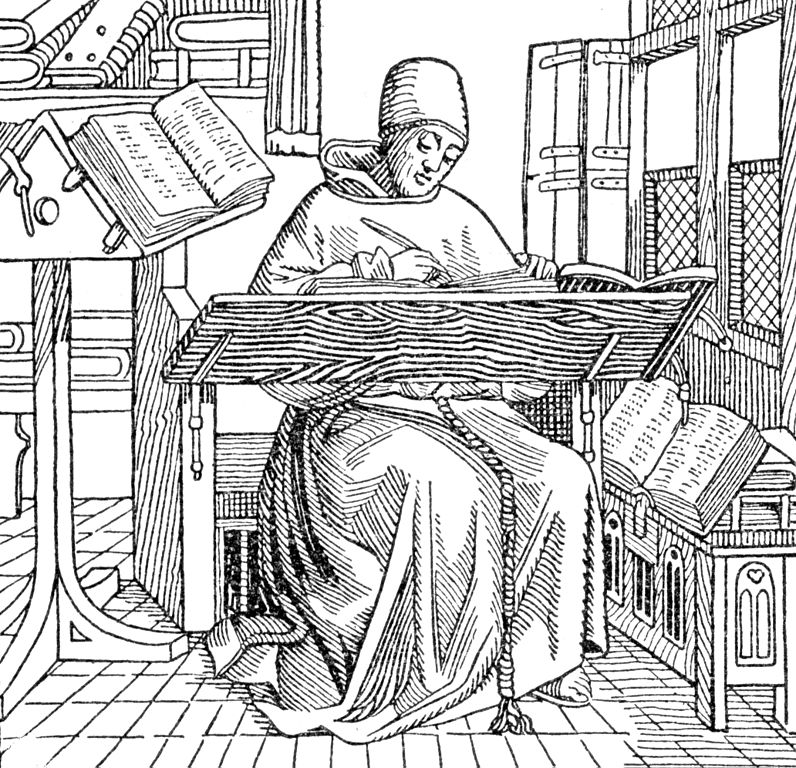
\includegraphics[width=\linewidth,keepaspectratio]{796px-Monkcopyistwoodcut} \\
    \tiny Wikimedia Commons
  \end{minipage}
\end{frame}

\begin{frame}
  \centering
  \dots\ to PowerPoint Syndrome \\
  \begin{minipage}{\linewidth}
    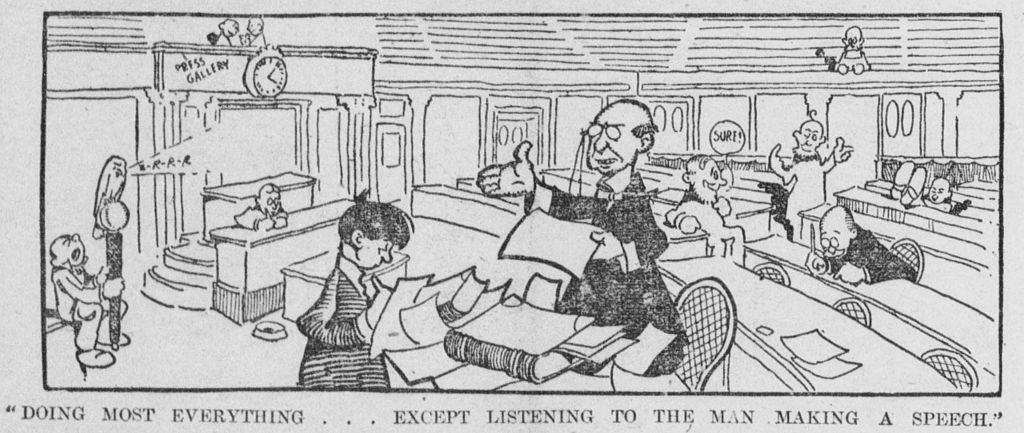
\includegraphics[width=\linewidth,keepaspectratio]{Satterfield_watches_Congress_be_boring} \\
    \tiny Wikimedia Commons
  \end{minipage}
\end{frame}

\begin{frame}
  \begin{center}
    \textbf{Late 2000s}
  \end{center}
  \begin{center}
    The classroom is obsolete! \\
    \emph{e-learning} is the future!
  \end{center}
\end{frame}

\begin{frame}
  \begin{center}
    \textbf{Pendulum is swinging back}
  \end{center}
  \begin{center}
    Students like to meet their teacher \\
    \pause
    \dots\ provided it's worth it.
  \end{center}
\end{frame}

\begin{frame}[standout]
  Disclaimer \\
  \bigskip

  I am not a specialist.

  Just an ordinary professor\dots \\
  with some experience
\end{frame}

\section{Blended Learning: Definition}

\begin{frame}
  \frametitle{Garrison and Vaughan (2008)}

  \begin{quote}
    Thoughtful fusion of face-to-face and online learning
    experiences [\dots] optimally integrated such that the strengths
    of each are blended into a unique learning experience congruent
    with the context and intended educational purpose.
  \end{quote}
\end{frame}

\begin{frame}
  \frametitle{Models of Blended Learning}

  \begin{description}[style=nextline]
  \item[Rotation model] Online engagement embedded within face-to-face
    forms of instruction in a cyclical manner
  \item[Flex model] Multiple students engaged primarily online, but
    under the supervision of a teacher who is physically present
  \item[Self-blending model] Students choose different courses to take
    independently, but do so in a setting where a supervising teacher
    and other students are co-present
  \item[\alert<2>{Enriched-virtual model}] Online, virtual experiences are seen
    as being enriched only periodically through arrangements of
    physical co-presence
  \end{description}
\end{frame}

\begin{frame}
  \frametitle{Continuum of Technology-Based Learning}

  \centering
  \begin{minipage}{0.75\linewidth}
    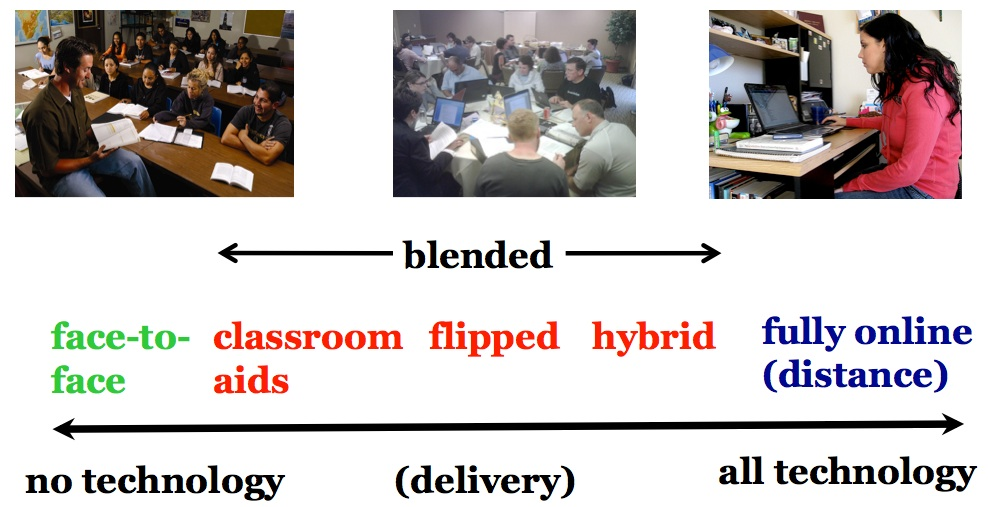
\includegraphics[width=\linewidth,keepaspectratio]{Continuum-of-technology-based-teaching-2} \\
    \tiny A.W. (Tony) Bates,
    \href{https://opentextbc.ca/teachinginadigitalage/}{Teaching in a Digital Age}
  \end{minipage}
  \vfill
  \mbox{}

  \only<2->{
    \begin{textblock*}{40mm}[1,0](85mm,80mm)
      \small\raggedleft%
      lectures prepared online before meeting in class
    \end{textblock*}
    \begin{textblock*}{0mm}(80mm,78mm)
      \setlength{\unitlength}{1mm}
      \begin{picture}(0,0)
        \put(-8,21){\framebox(16,6.5)[bl]{}}
        \put(0,0){\line(0,1){21}}
      \end{picture}
    \end{textblock*}}

  \only<3->{
    \begin{textblock*}{60mm}(92mm,80mm)
      \small\raggedright%
      majority of learning online, class only for very specific
      face-to-face teaching that cannot be done satisfactorily online
    \end{textblock*}
    \begin{textblock*}{0mm}(97mm,78mm)
      \setlength{\unitlength}{1mm}
      \begin{picture}(0,0)
        \put(-8,21){\framebox(16,6.5)[bl]{}}
        \put(0,0){\line(0,1){21}}
      \end{picture}
    \end{textblock*}}
\end{frame}

%%% Local Variables:
%%% mode: latex
%%% TeX-engine: xetex
%%% TeX-master: "atc-2017-blended-learning"
%%% End:
